\documentclass[11pt]{article}
\usepackage{algorithm2e}
\usepackage[italian]{babel}
\usepackage{ragged2e}
\usepackage{amsfonts, amssymb, amsmath}
\usepackage{cancel}
\usepackage{float}
\usepackage{mathtools}
\usepackage{hyperref}
\usepackage{subfig}
\usepackage[margin={3cm, 1.5cm}, includefoot]{geometry}
\justifying

\hypersetup{
    colorlinks=true,
    linkcolor=black,
    filecolor=black,      
    urlcolor=black,
}

\tolerance=1
\emergencystretch=\maxdimen
\hyphenpenalty=10000
\hbadness=10000

\begin{document}
\begin{titlepage}
    \begin{center}
        \vspace*{3.0cm}
            
        \Huge
        \textbf{Map Connectivity}
            
        \vspace{0.3cm}
        \LARGE
        Relazione progetto

        \vspace{1.5cm}
          
        \begin{minipage}[t]{0.47\textwidth}
            \begin{center}
                {\large{\bf Cheikh Ibrahim $\cdot$ Zaid}}\\
                {\large Matricola: \texttt{0000974909}} \\
                {\large{\href{mailto:zaid.cheikhibrahim@studio.unibo.it}{\texttt{zaid.cheikhibrahim@studio.unibo.it}}}}
            \end{center}
    
            \end{minipage}
            \hfill
            \begin{minipage}[t]{0.47\textwidth}\raggedleft
            \begin{center}
                {\large{\bf Paris $\cdot$ Manuel}}\\
                {\large Matricola: \texttt{0000997526}}
                {\large{\href{mailto:manuel.paris@studio.unibo.it}{\texttt{manuel.paris@studio.unibo.it}}}}
            \end{center}
        \end{minipage}
            
        \vspace{6cm}
            
        Anno accademico\\
        $2022 - 2023$
            
        \vspace{0.8cm}
            
            
        \Large
        Corso di Laboratorio di Applicazioni Mobili\\
        Alma Mater Studiorum $\cdot$ Università di Bologna\\
            
    \end{center}
\end{titlepage}
\pagebreak
\pagenumbering{gobble} 
\tableofcontents
\pagebreak
\pagenumbering{arabic} 

\section{Introduzione}
L'applicazione \texttt{MapConnectivity} è un software sviluppato in Kotlin che permette di registrare e visualizzare su una mappa, tramite una griglia a riquadri e uno schema di colori prefissato (rosso = pessimo, giallo = medio, verde = ottimo), le misurazioni della potenza del segnale LTE, Wi-Fi e il rumore misurato in dB nella zona circostante. \\
È possibile effettuare misure in tre modi diversi:
\begin{enumerate}
    \item Manualmente - tramite la pressione di un bottone,
    \item Automaticamente - viene effettuata una misura ogni volta che l'utente entra in un nuovo riquadro,
    \item Periodicamente - viene effettuata una misura ogni intervallo scelto dall'utente.
\end{enumerate}
Inoltre, è possibile scambiare le proprie misure con un altro dispositivo tramite file o Bluetooth.
\subsection{Main Activity}
\begin{minipage}[t]{0.65\textwidth}
La schermata principale dell'applicazione (Figura \ref{fig:mainActivity}). \\
All'avvio, una volta concessi i permessi richiesti, viene mostrata la mappa con la griglia. Inoltre è presente un indicatore che mostra la modalità attuale di visualizzazione, ovvero se i colori mostrati sulla griglia si riferiscono a misure relative a LTE, Wi-Fi o dB. \\
Il bottone \texttt{Misura} effettua una misura calcolando l'intensità del valore LTE, Wi-Fi e dB localizzandoli nella posizione attuale dell'utente. \\
Sotto la mappa sono presenti, inoltre, due bottoni che portano alle altre schermate dell'applicazione: Impostazioni (Capitolo \ref{sec:settingsActivity}) e Scambio dati (Capitolo \ref{sec:swapActivity}). \\ \\
Premendo su un riquadro (Figura \ref{fig:showMore}), è possibile mostrare una schermata riepilogativa di tutte le misure presenti in quel riquadro. Selezionando una specifica misura, è possibile visualizzarne nel dettaglio i dati oppure eliminarla.
\end{minipage} \hfill
\begin{minipage}[t]{0.25\textwidth}
    \begin{figure}[H]
        \centering
        \vspace*{-0.7cm}
        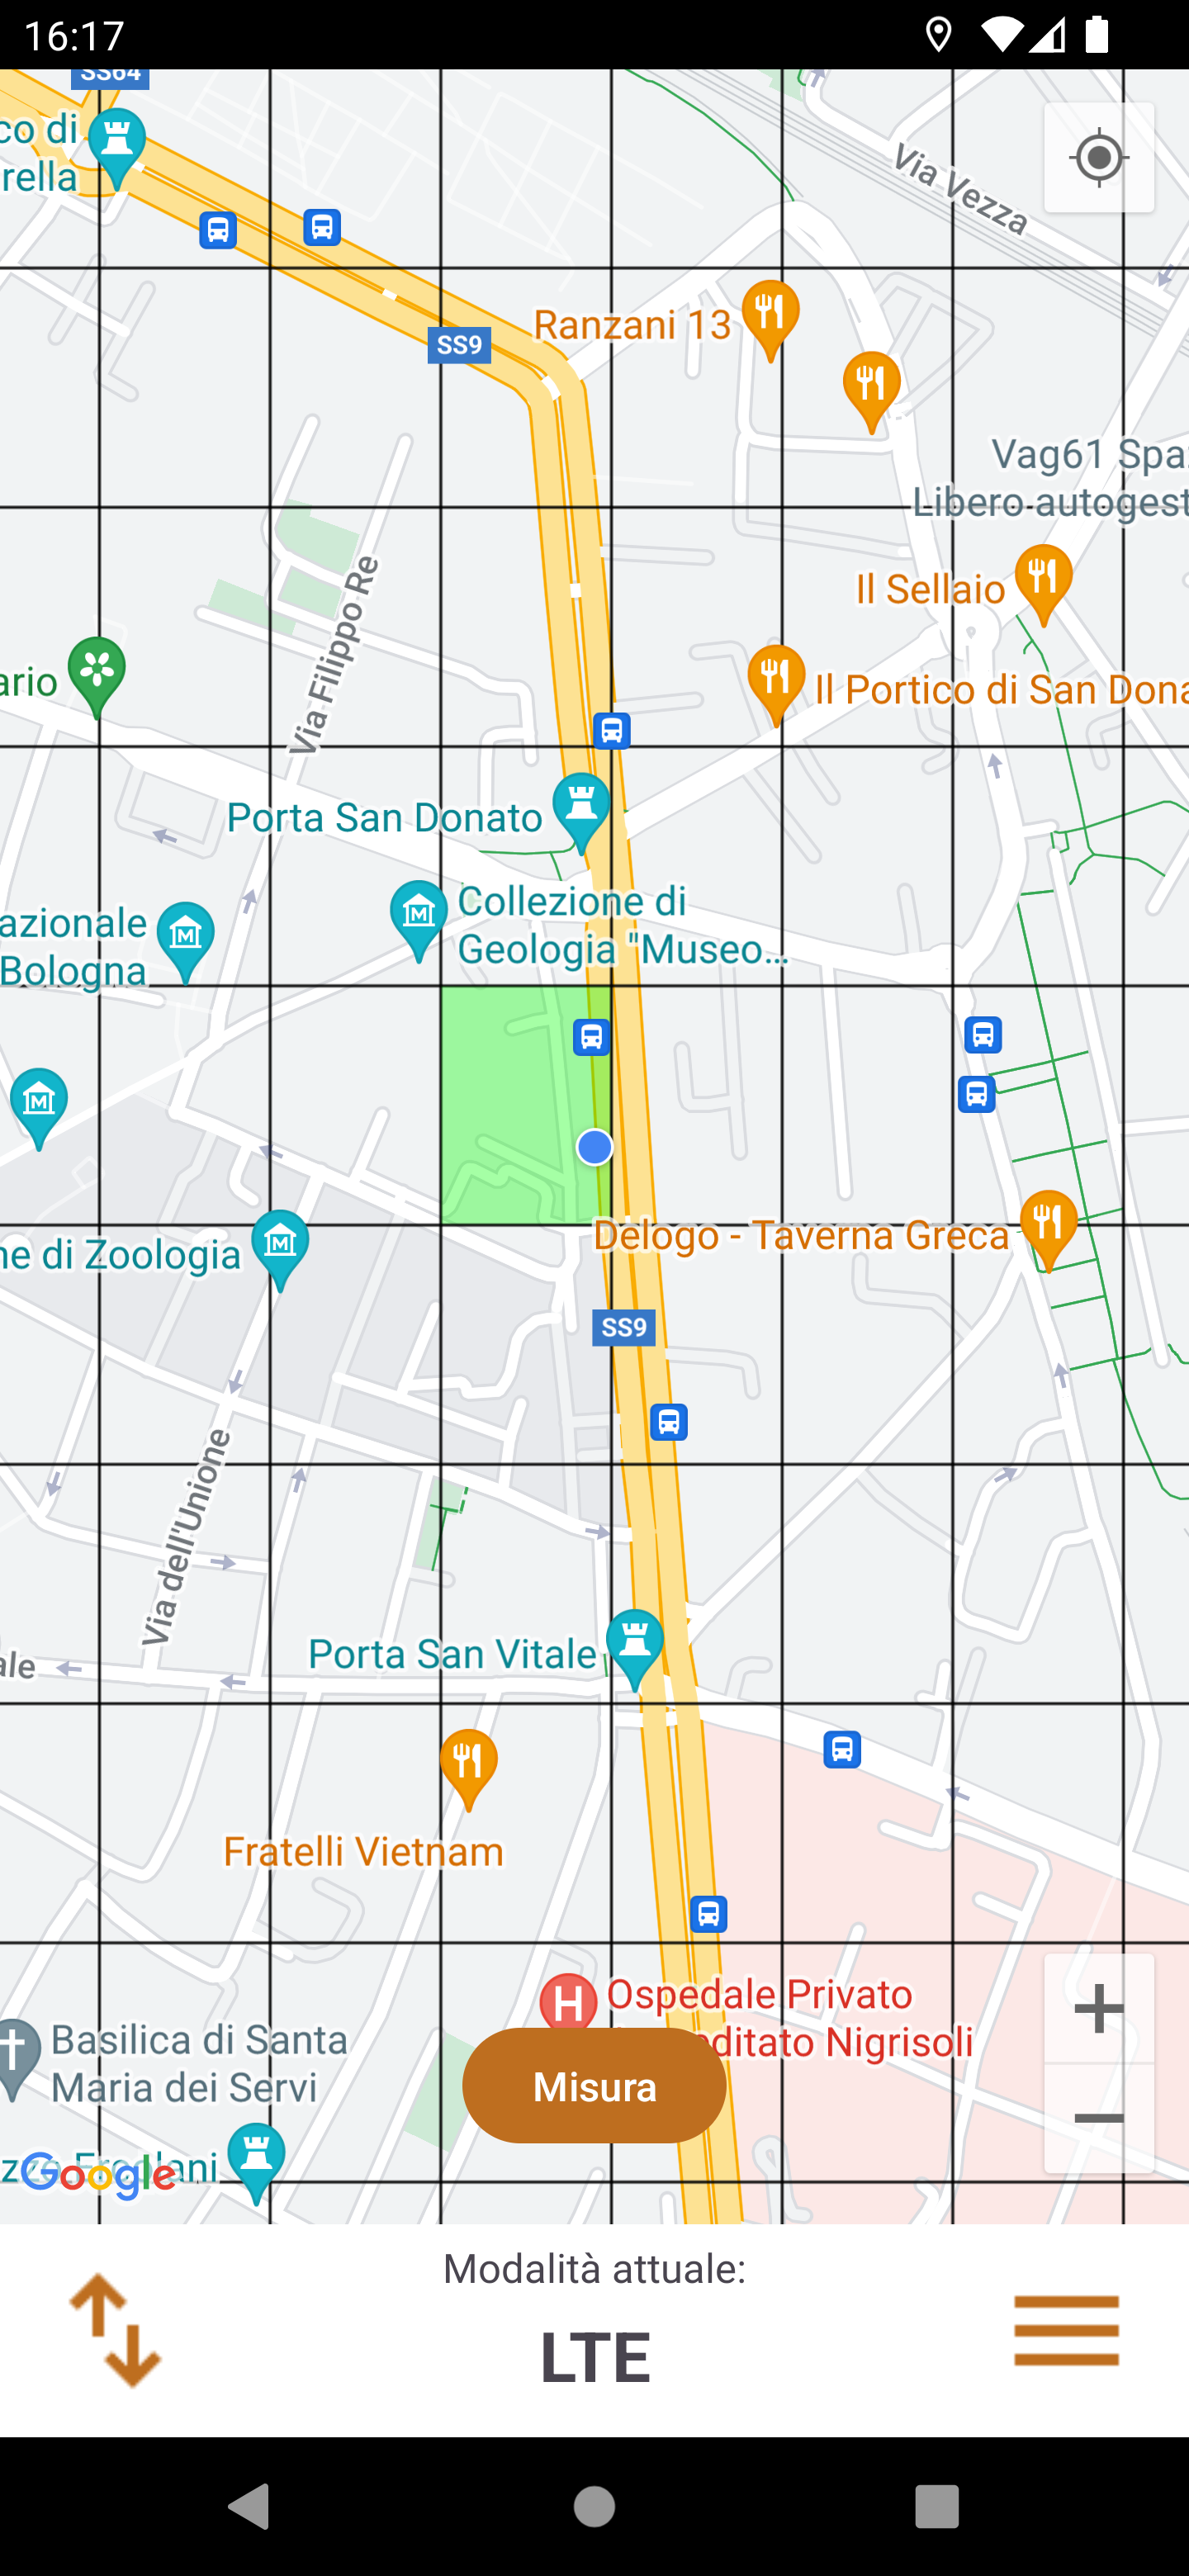
\includegraphics[width=\textwidth]{img/mainActivity.png}
        \caption{Schermata principale}
        \label{fig:mainActivity}
    \end{figure}
\end{minipage}
\begin{figure}[H] 
    \centering
    \subfloat[Premendo su un riquadro]{%
        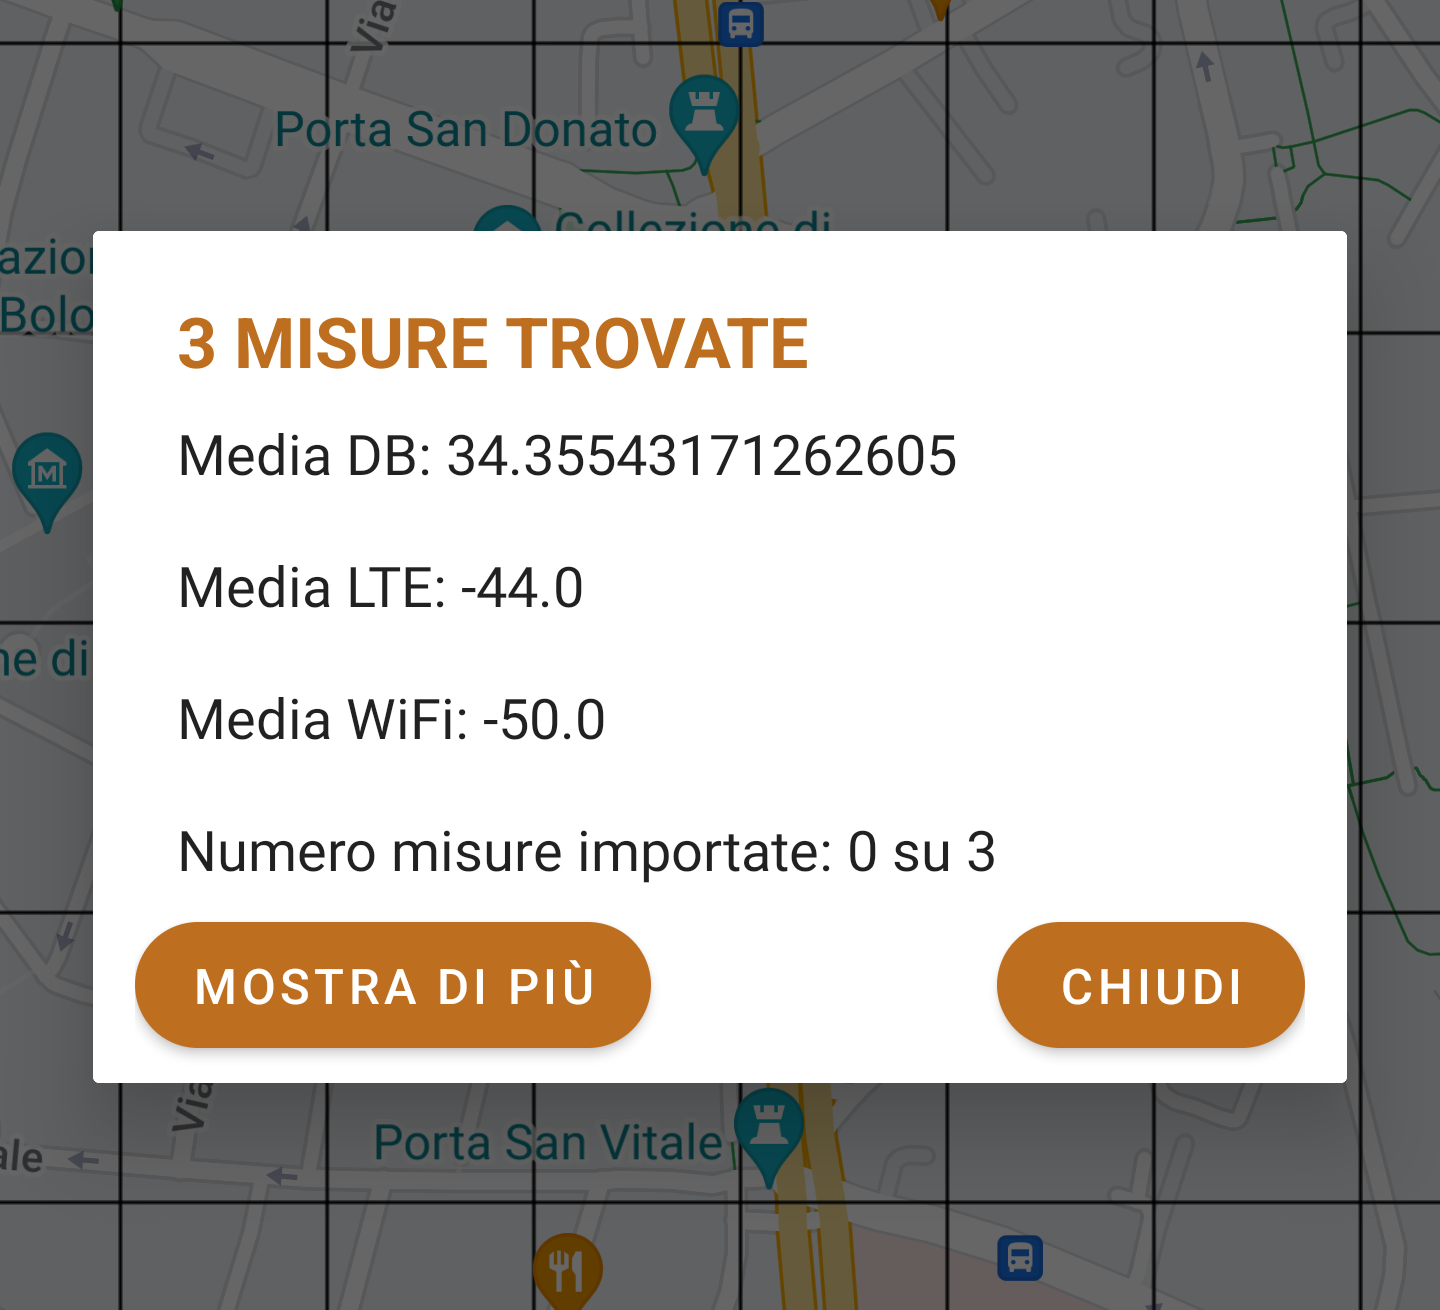
\includegraphics[width=0.3\textwidth]{img/showMore1.png}%
        \label{fig:showMore1}%
        }%
    \hfill%
    \subfloat[Premendo su "Mostra di più"]{%
        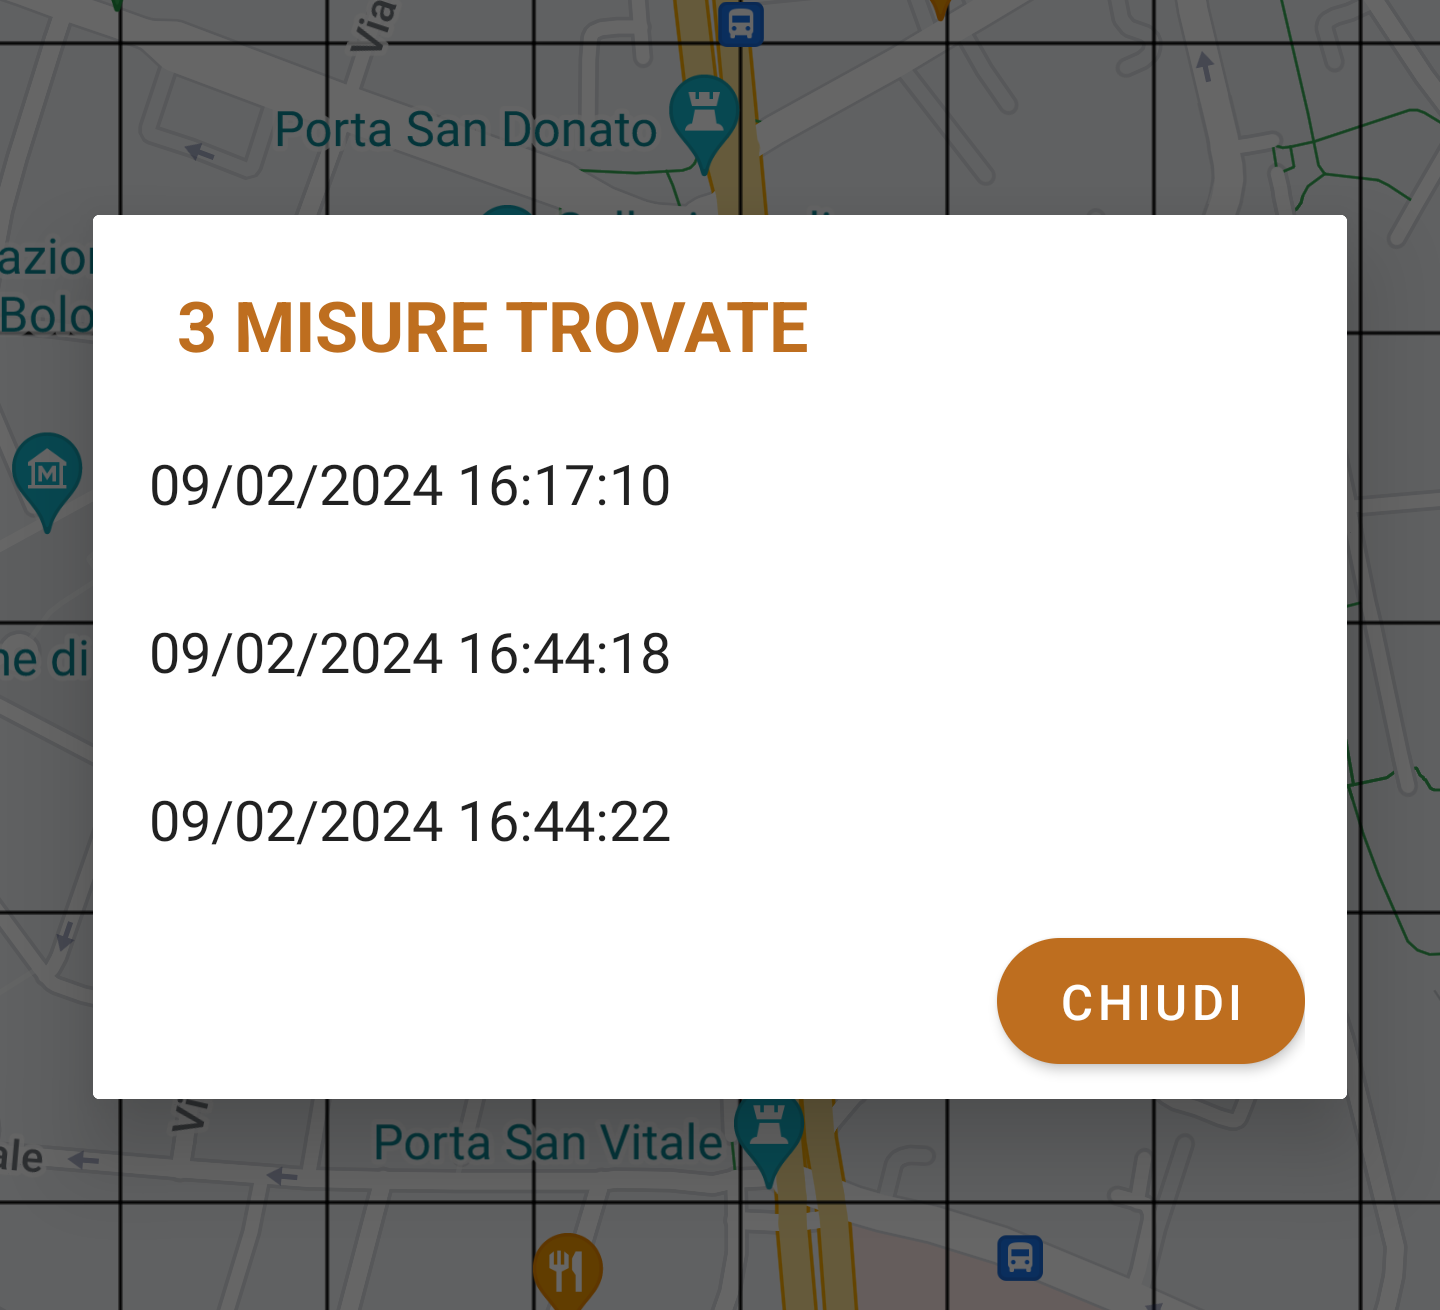
\includegraphics[width=0.3\textwidth]{img/showMore2.png}%
        \label{fig:showMore2}%
        }%
    \hfill%
    \subfloat[Premendo su una misura]{%
        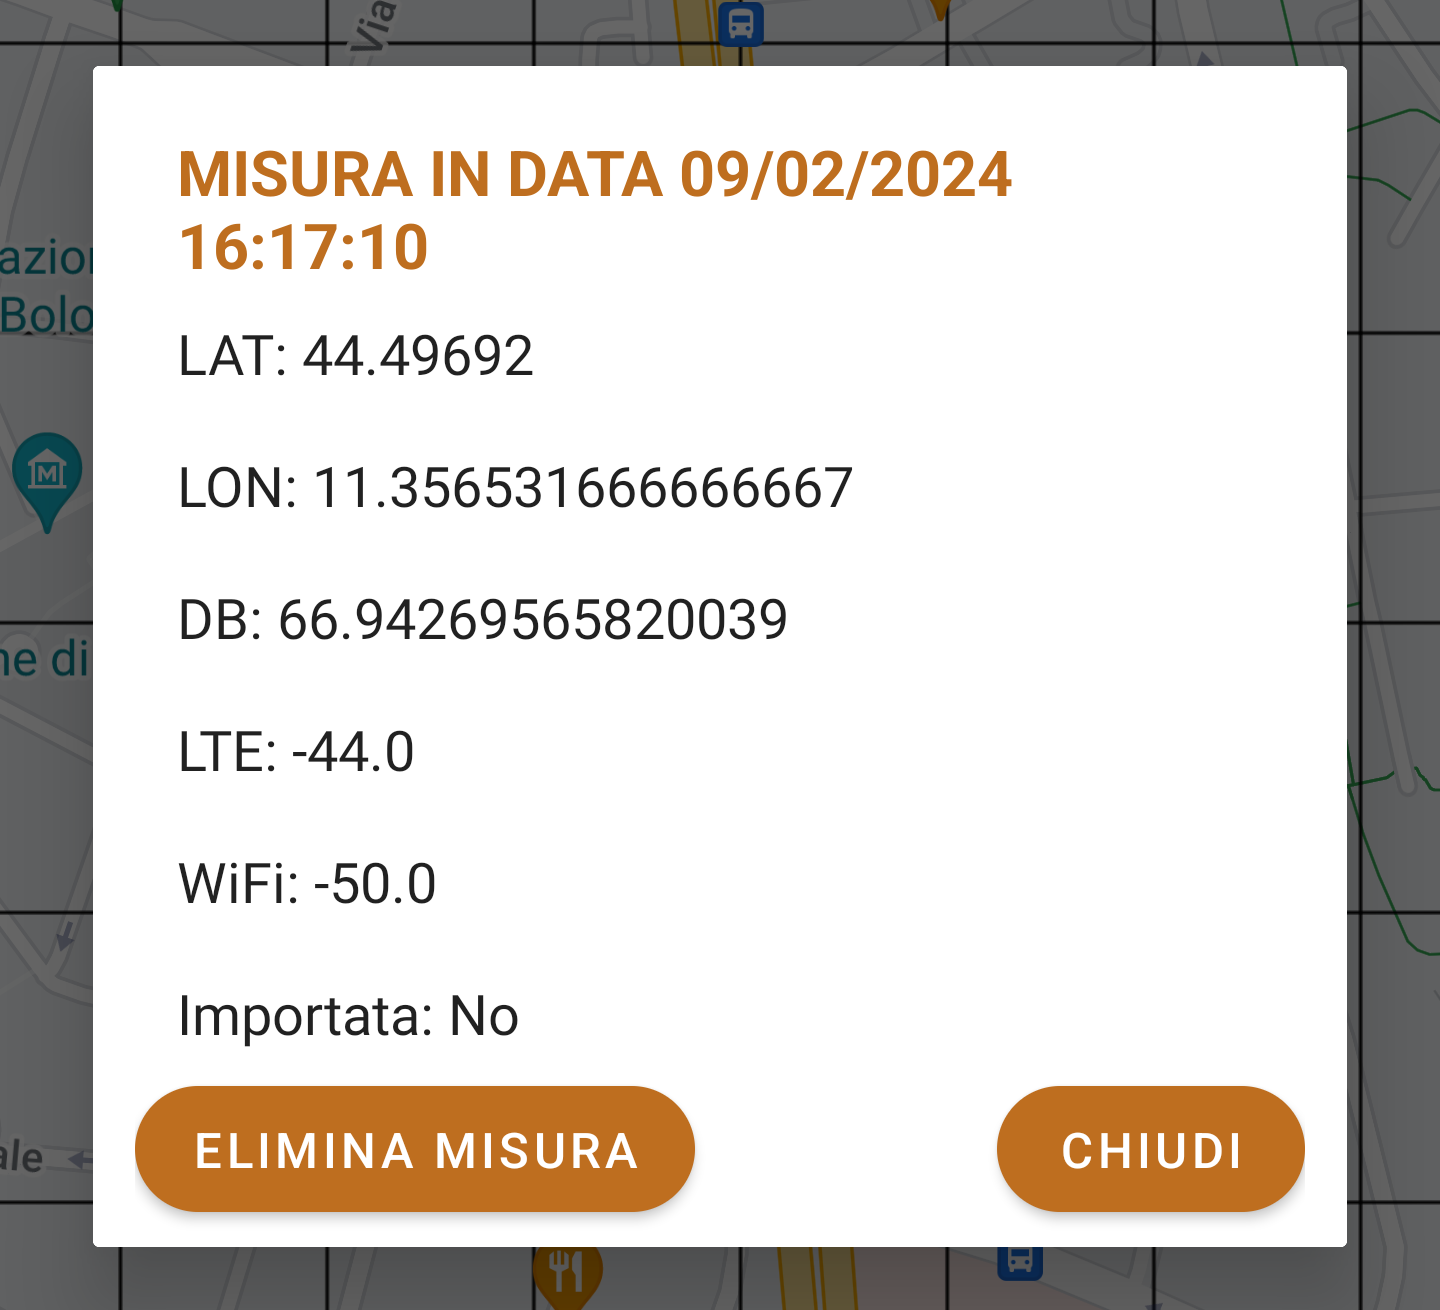
\includegraphics[width=0.3\textwidth]{img/showMore3.png}%
        \label{fig:showMore3}%
        }%

    \caption{Schermata riepilogativa}
    \label{fig:showMore}
\end{figure}
\pagebreak
\subsection{Settings Activity}
\label{sec:settingsActivity}
Schermata contenente le impostazioni per le preferenze e modalità di misurazione (Figura \ref{fig:settingsActivity}). \\
L'utente ha la possibilità di scegliere:
\begin{itemize}
    \item Il tema, tra chiaro, scuro e predefinito del S.O.,
    \item Il parametro di visualizzazione, tra LTE, Wi-Fi o dB,
    \item Se mostrare o no le misure importate,
    \item Di attivare una particolare modalità di scansione, tra automatica, periodica e periodica in background,
    \item L'intervallo di scansione, ovvero ogni quanto effettuare una scansione quando è attiva quella periodica,
    \item La durata della discoverabilità, ovvero quanto rimanere discoverabile durante l'esportazione via Bluetooth,
    \item Di limitare le misure da tenere in considerazione da visualizzare sulla mappa e in caso affermativo ne può specificare il numero,
    \item Di impostare delle soglie manuali per la visualizzazione dei colori su mappa,
    \item Di attivare la funzionalità di notifica quando si entra in un riquadro con misure non recenti al giorno odierno,
    \item Di cancellare le misure (tutte, solo quelle effettuate dall'utente o solo quelle importate).
\end{itemize}
\begin{figure}[H] 
    \centering
    \subfloat[]{%
        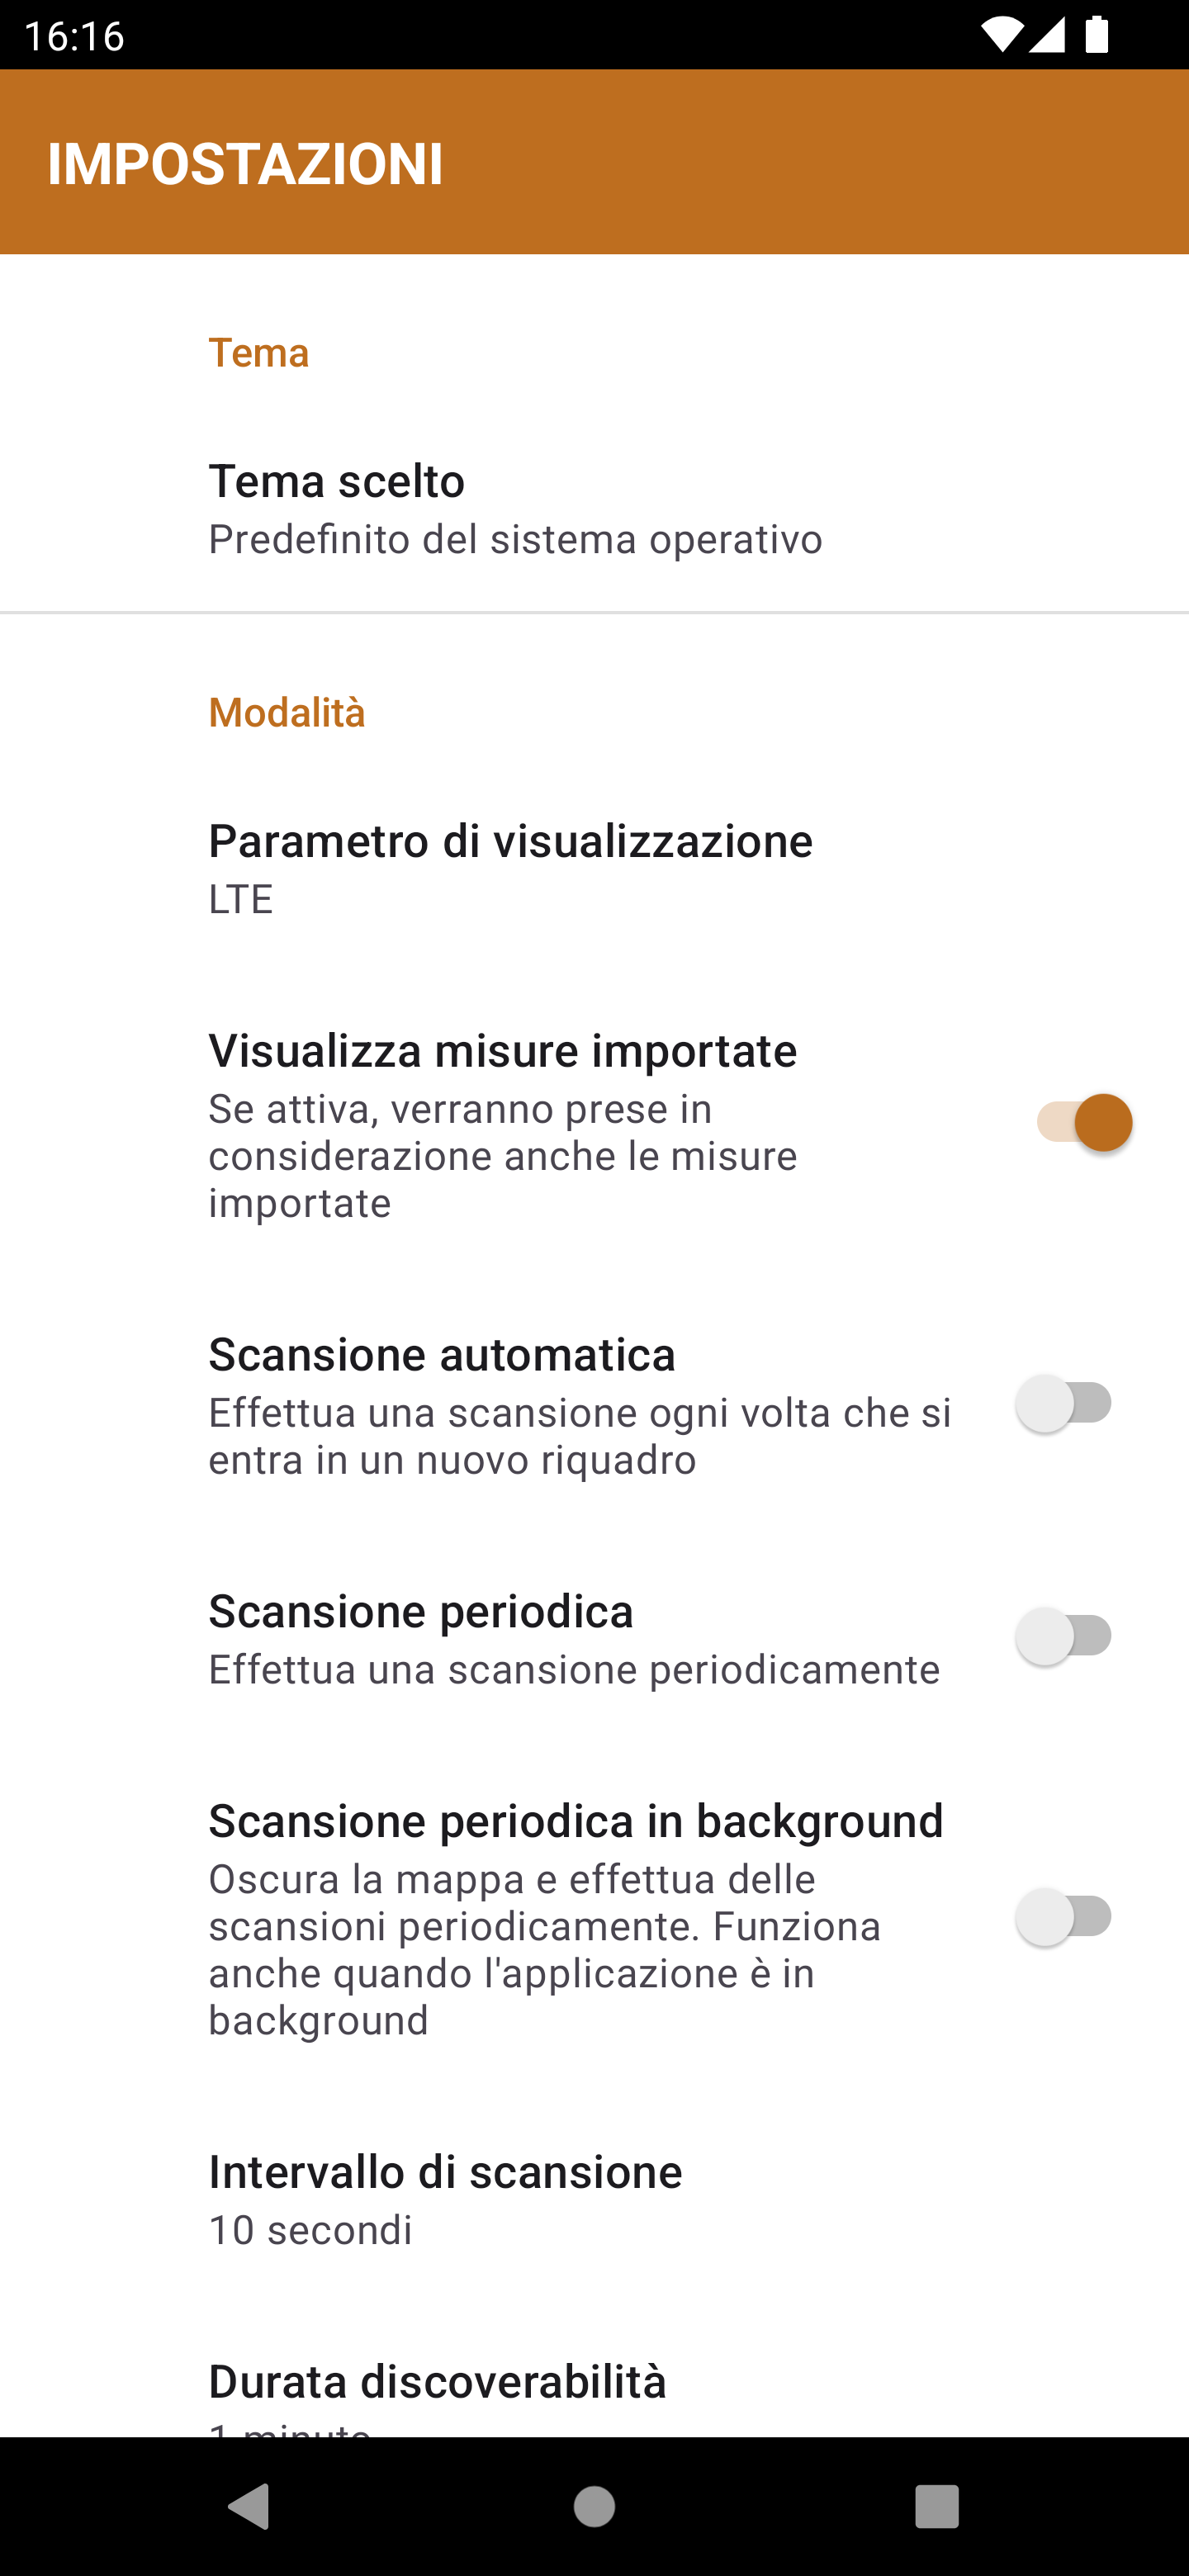
\includegraphics[width=0.3\textwidth]{img/settingsActivity1.png}%
        \label{fig:settingsActivity1}%
        }%
    \hfill%
    \subfloat[]{%
        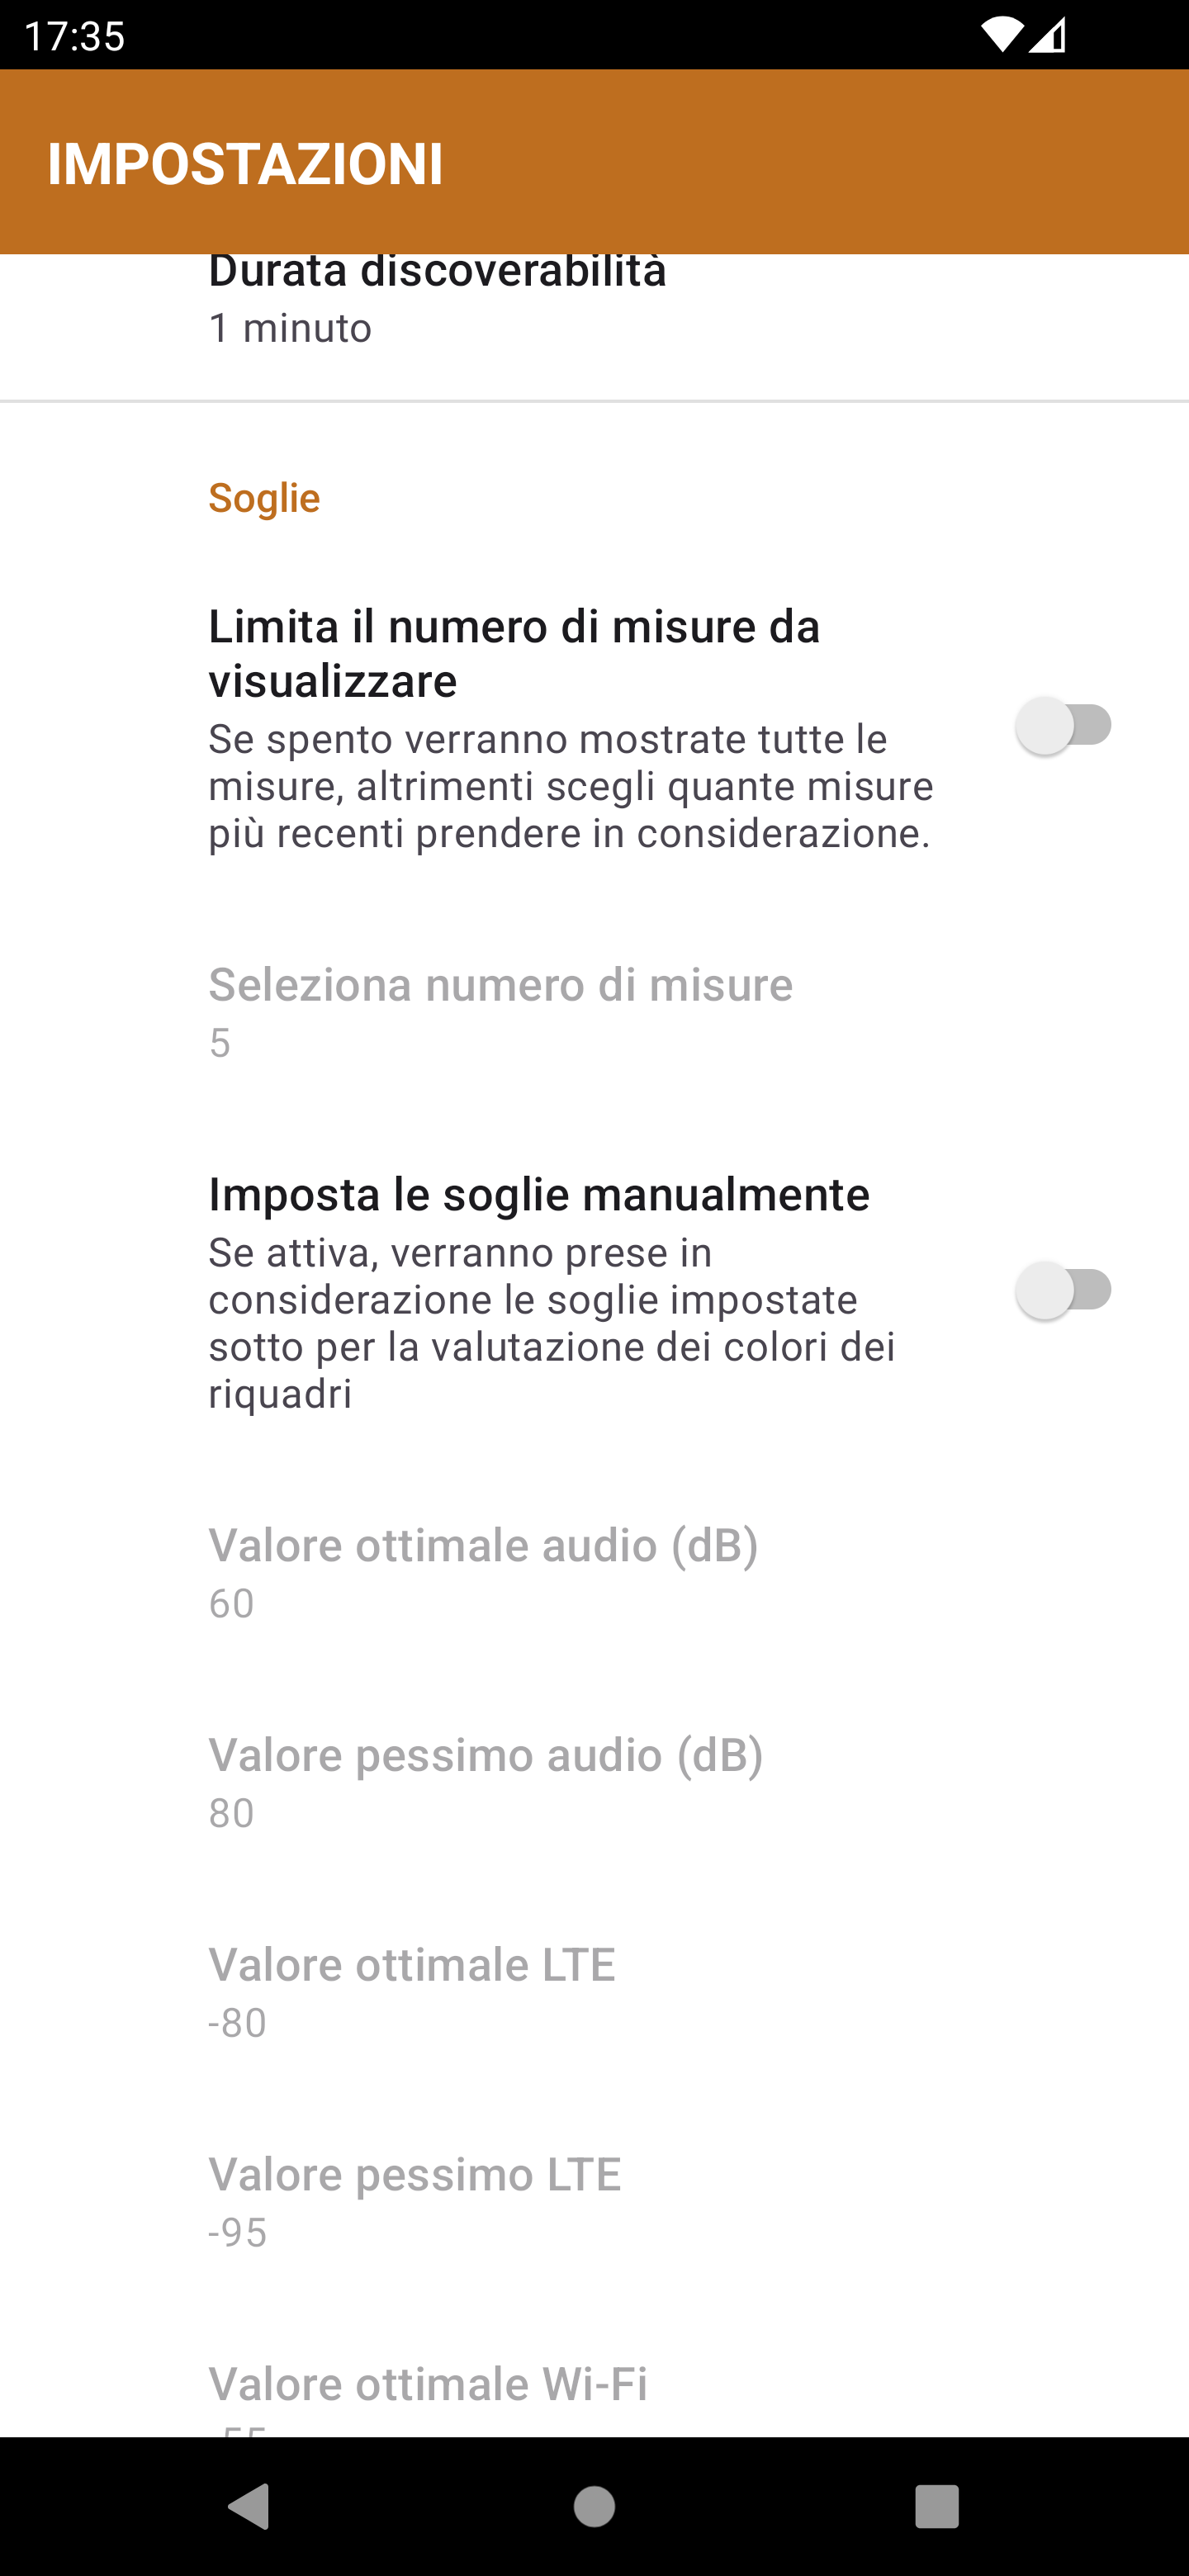
\includegraphics[width=0.3\textwidth]{img/settingsActivity2.png}%
        \label{fig:settingsActivity2}%
        }%
    \hfill%
    \subfloat[]{%
        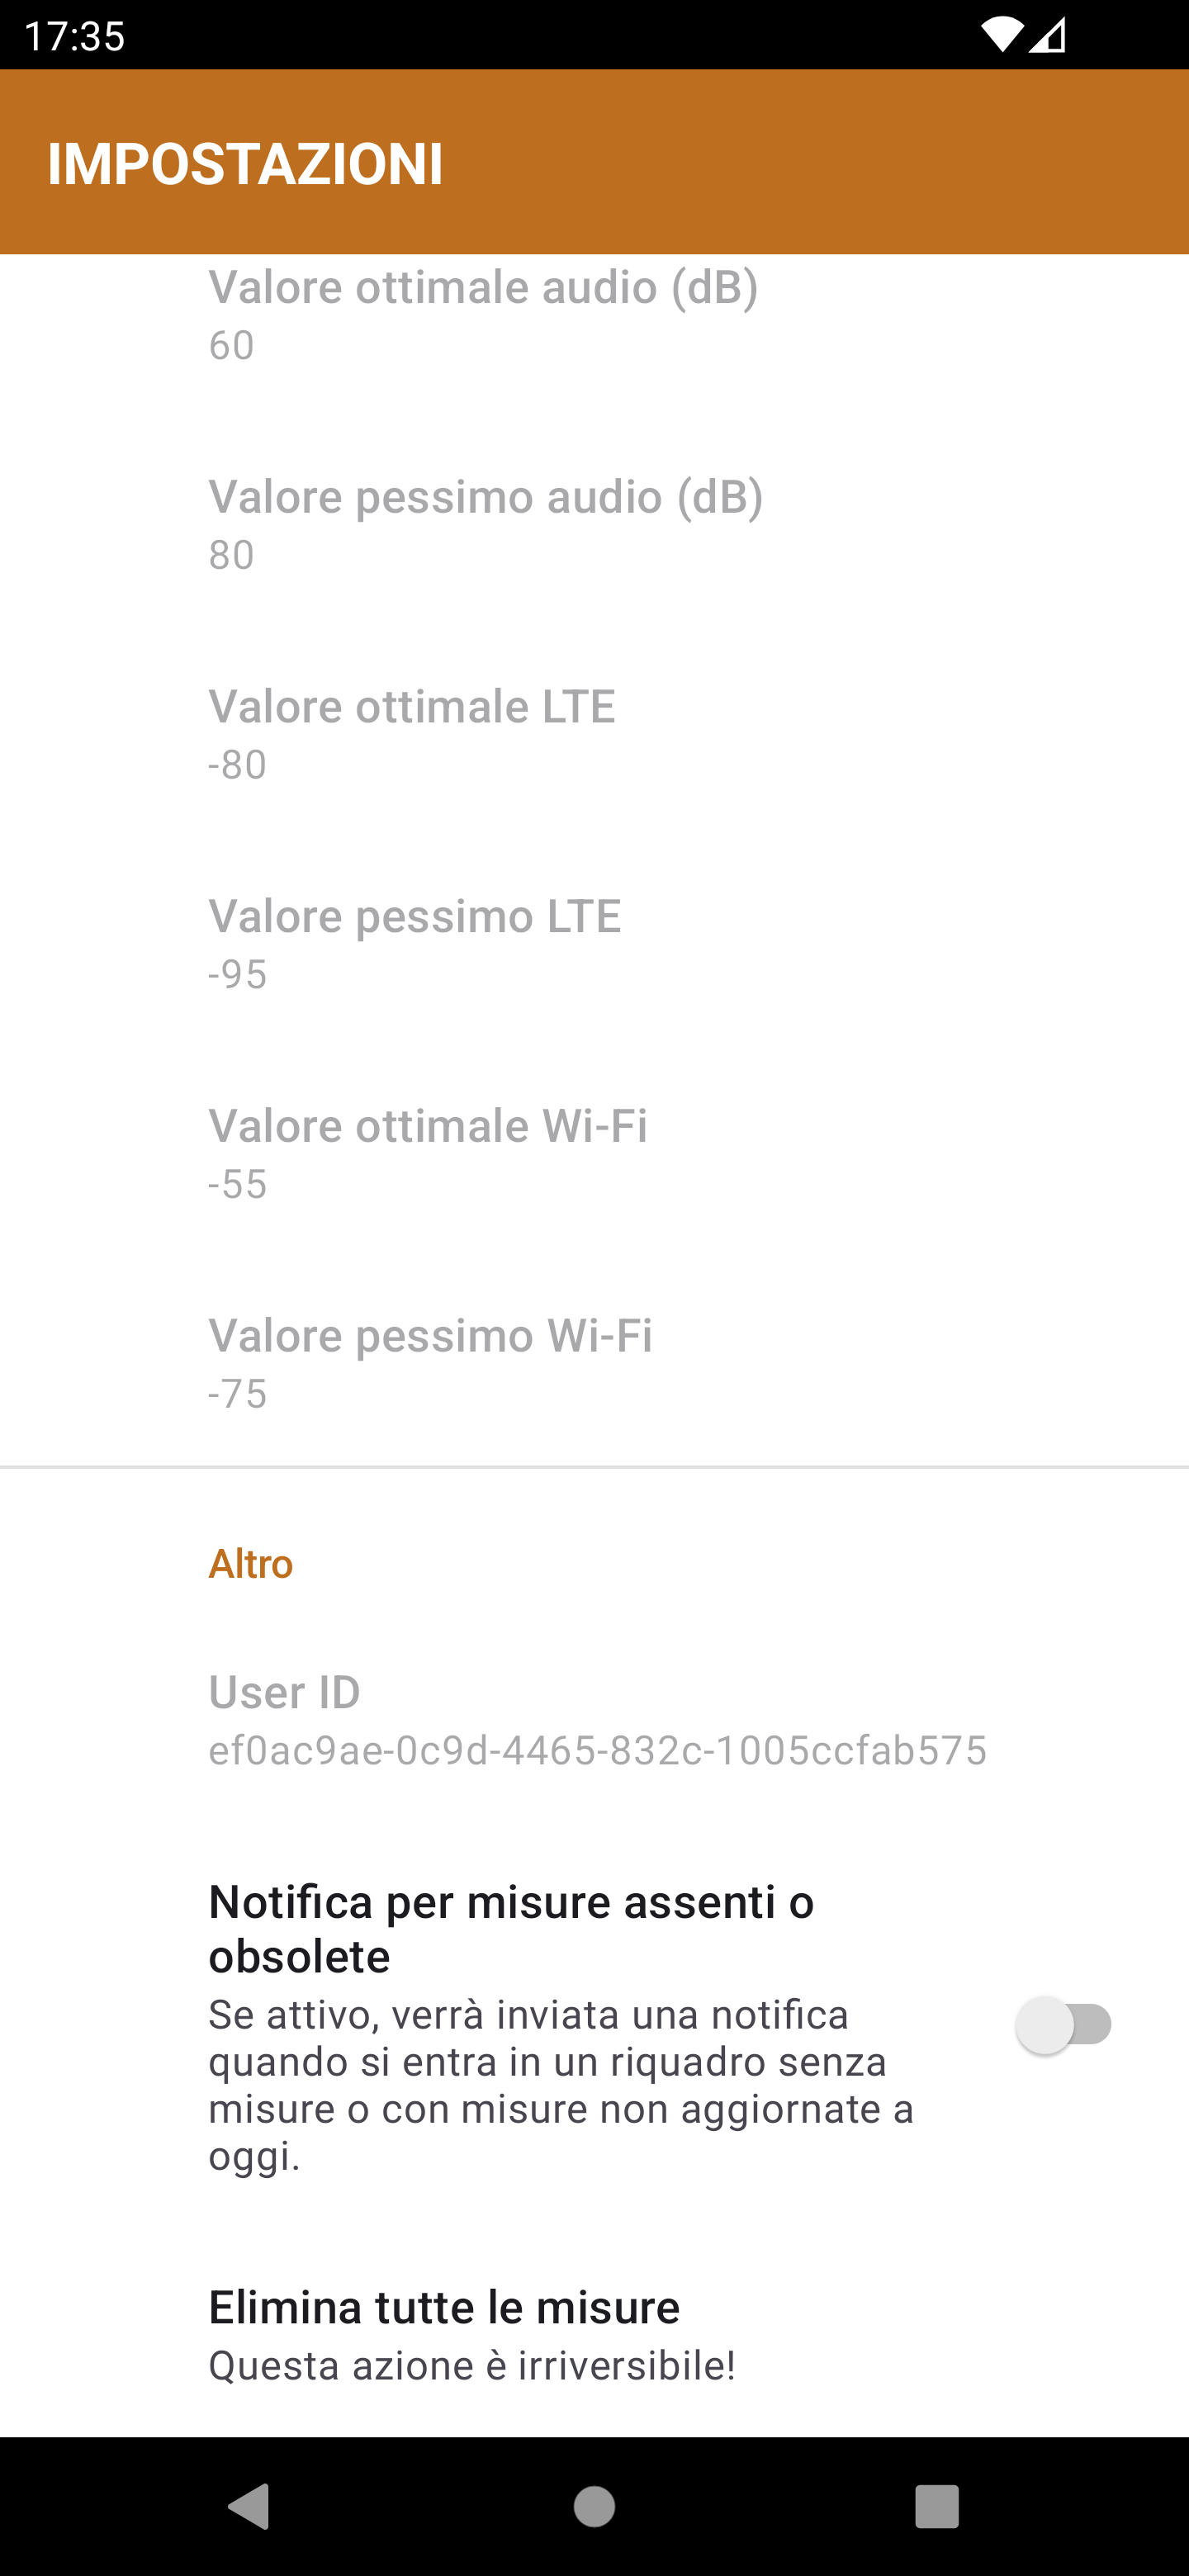
\includegraphics[width=0.3\textwidth]{img/settingsActivity3.png}%
        \label{fig:settingsActivity3}%
        }%

    \caption{Schermata delle impostazioni}
    \label{fig:settingsActivity}
\end{figure}
\pagebreak
\subsection{Swap Activity}
\label{sec:swapActivity}
Schermata contenente le opzioni di scambio dati (Figura \ref{fig:swapActivity}). \\
L'utente può scegliere di scambiare i dati con un altro dispositivo o tramite l'invio di file o tramite Bluetooth. \\
Ci sono quindi 4 opzioni:
\begin{itemize}
    \item Importazione da file: verrà chiesto di selezionare il file \texttt{.mapc} dall'archivio del dispositivo.
    \item Esportazione da file: verrà creato un file \texttt{export\_data-ora.mapc} contenente tutte le misure presenti nel database, tranne quelle importate, e verrà chiesto all'utente il modo di inviare tale file.
    \item Importazione da Bluetooth: verranno visualizzati i dispositivi nelle vicinanze discoverabili tramite Bluetooth e selezionandone uno verrà inizializzata la connessione per importare le misure automaticamente (Figura \ref{fig:importBluetooth}).
    \item Esportazione da Bluetooth: in base alla durata di discoverabilità presente nelle impostazioni, il dispositivo diventerà discoverabile dagli altri per quella durata e alla richiesta di importazione da parte di un dispositivo, gli invierà tutte le misure presenti nel database, tranne quelle importate (Figura \ref{fig:exportBluetooth}).
\end{itemize}
\begin{figure}[H] 
    \centering
    \subfloat[Schermata generale]{%
        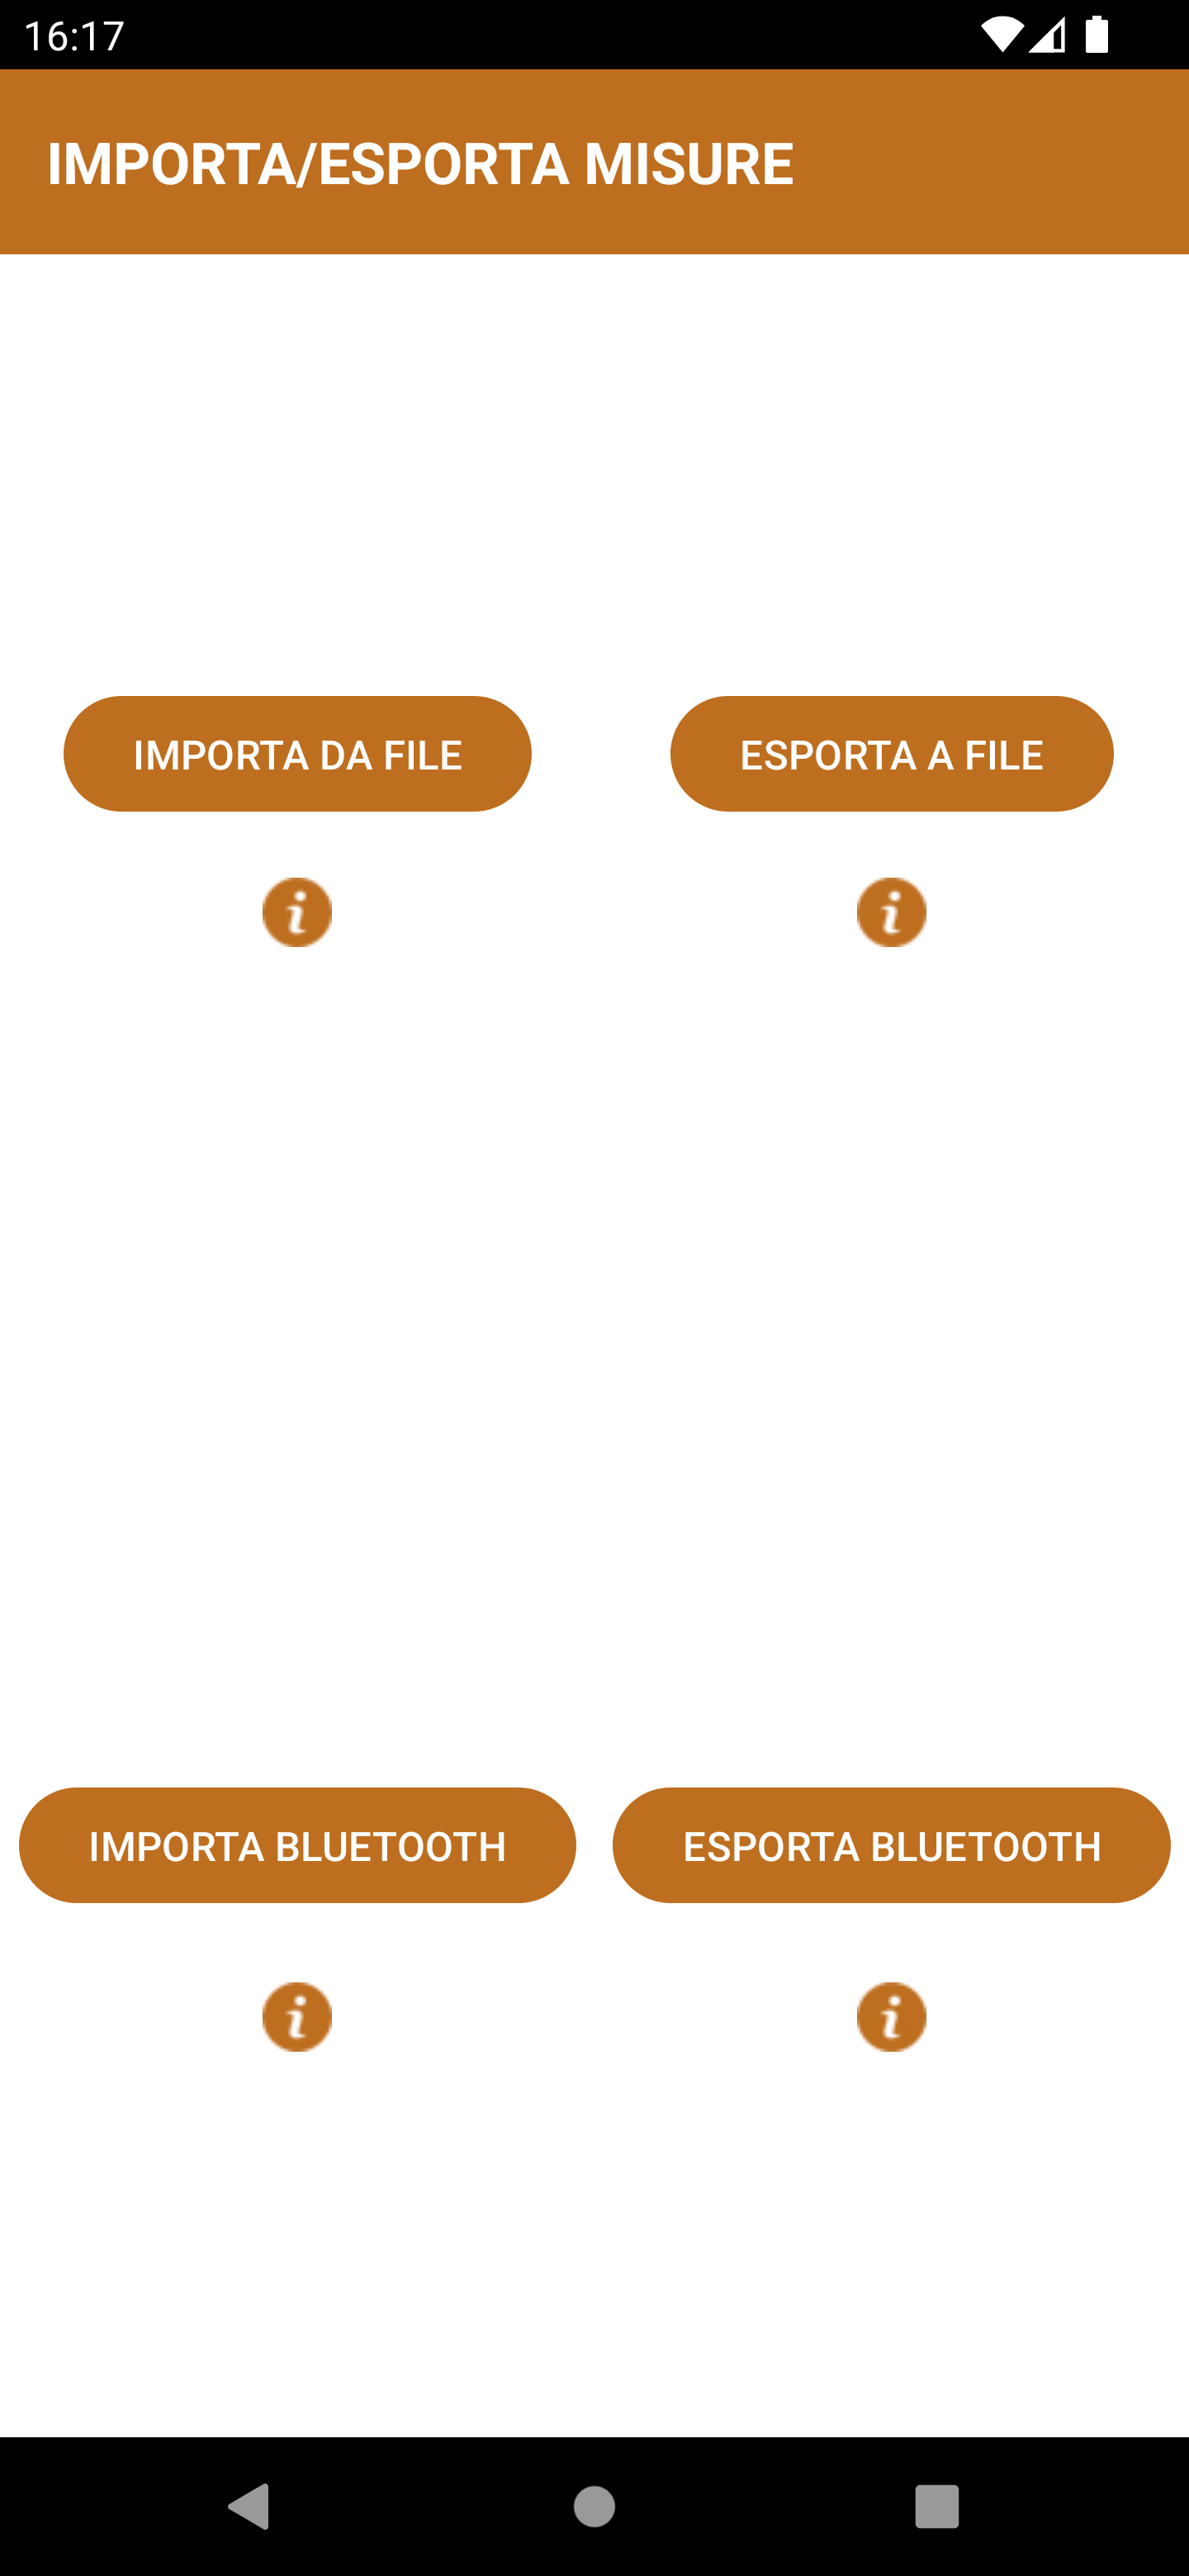
\includegraphics[width=0.3\textwidth]{img/swapActivity.png}%
        \label{fig:swapActivity}%
        }%
    \hfill%
    \subfloat[Schermata di importazione tramite Bluetooth]{%
        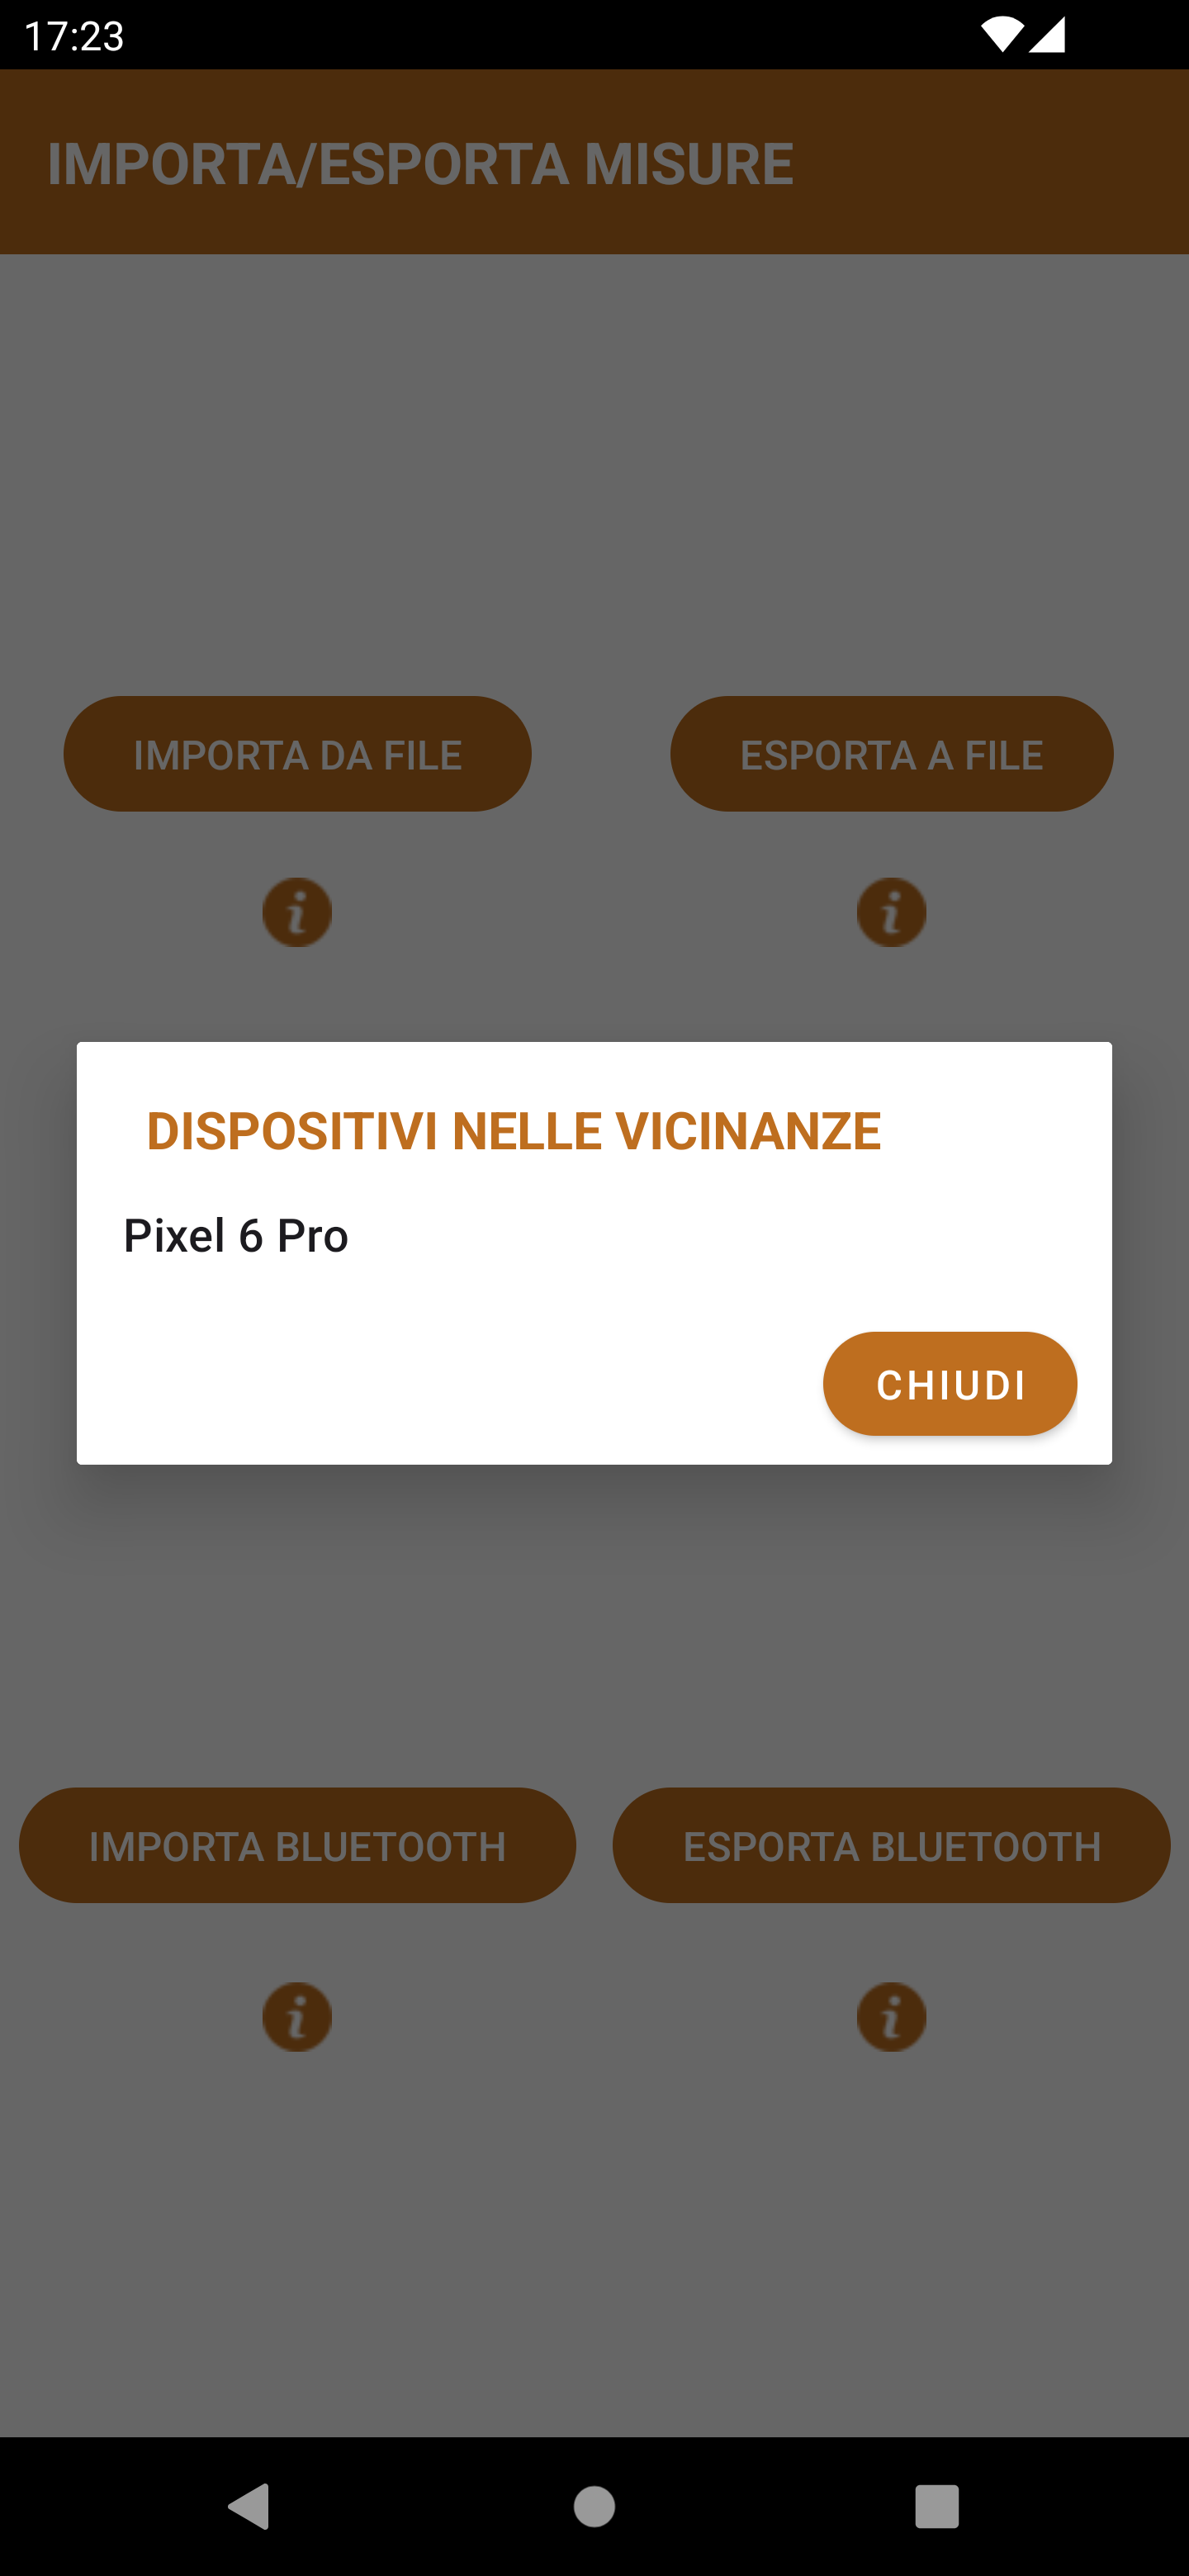
\includegraphics[width=0.3\textwidth]{img/importBluetooth.png}%
        \label{fig:importBluetooth}%
        }%
    \hfill%
    \subfloat[Schermata di esportazione tramite Bluetooth]{%
        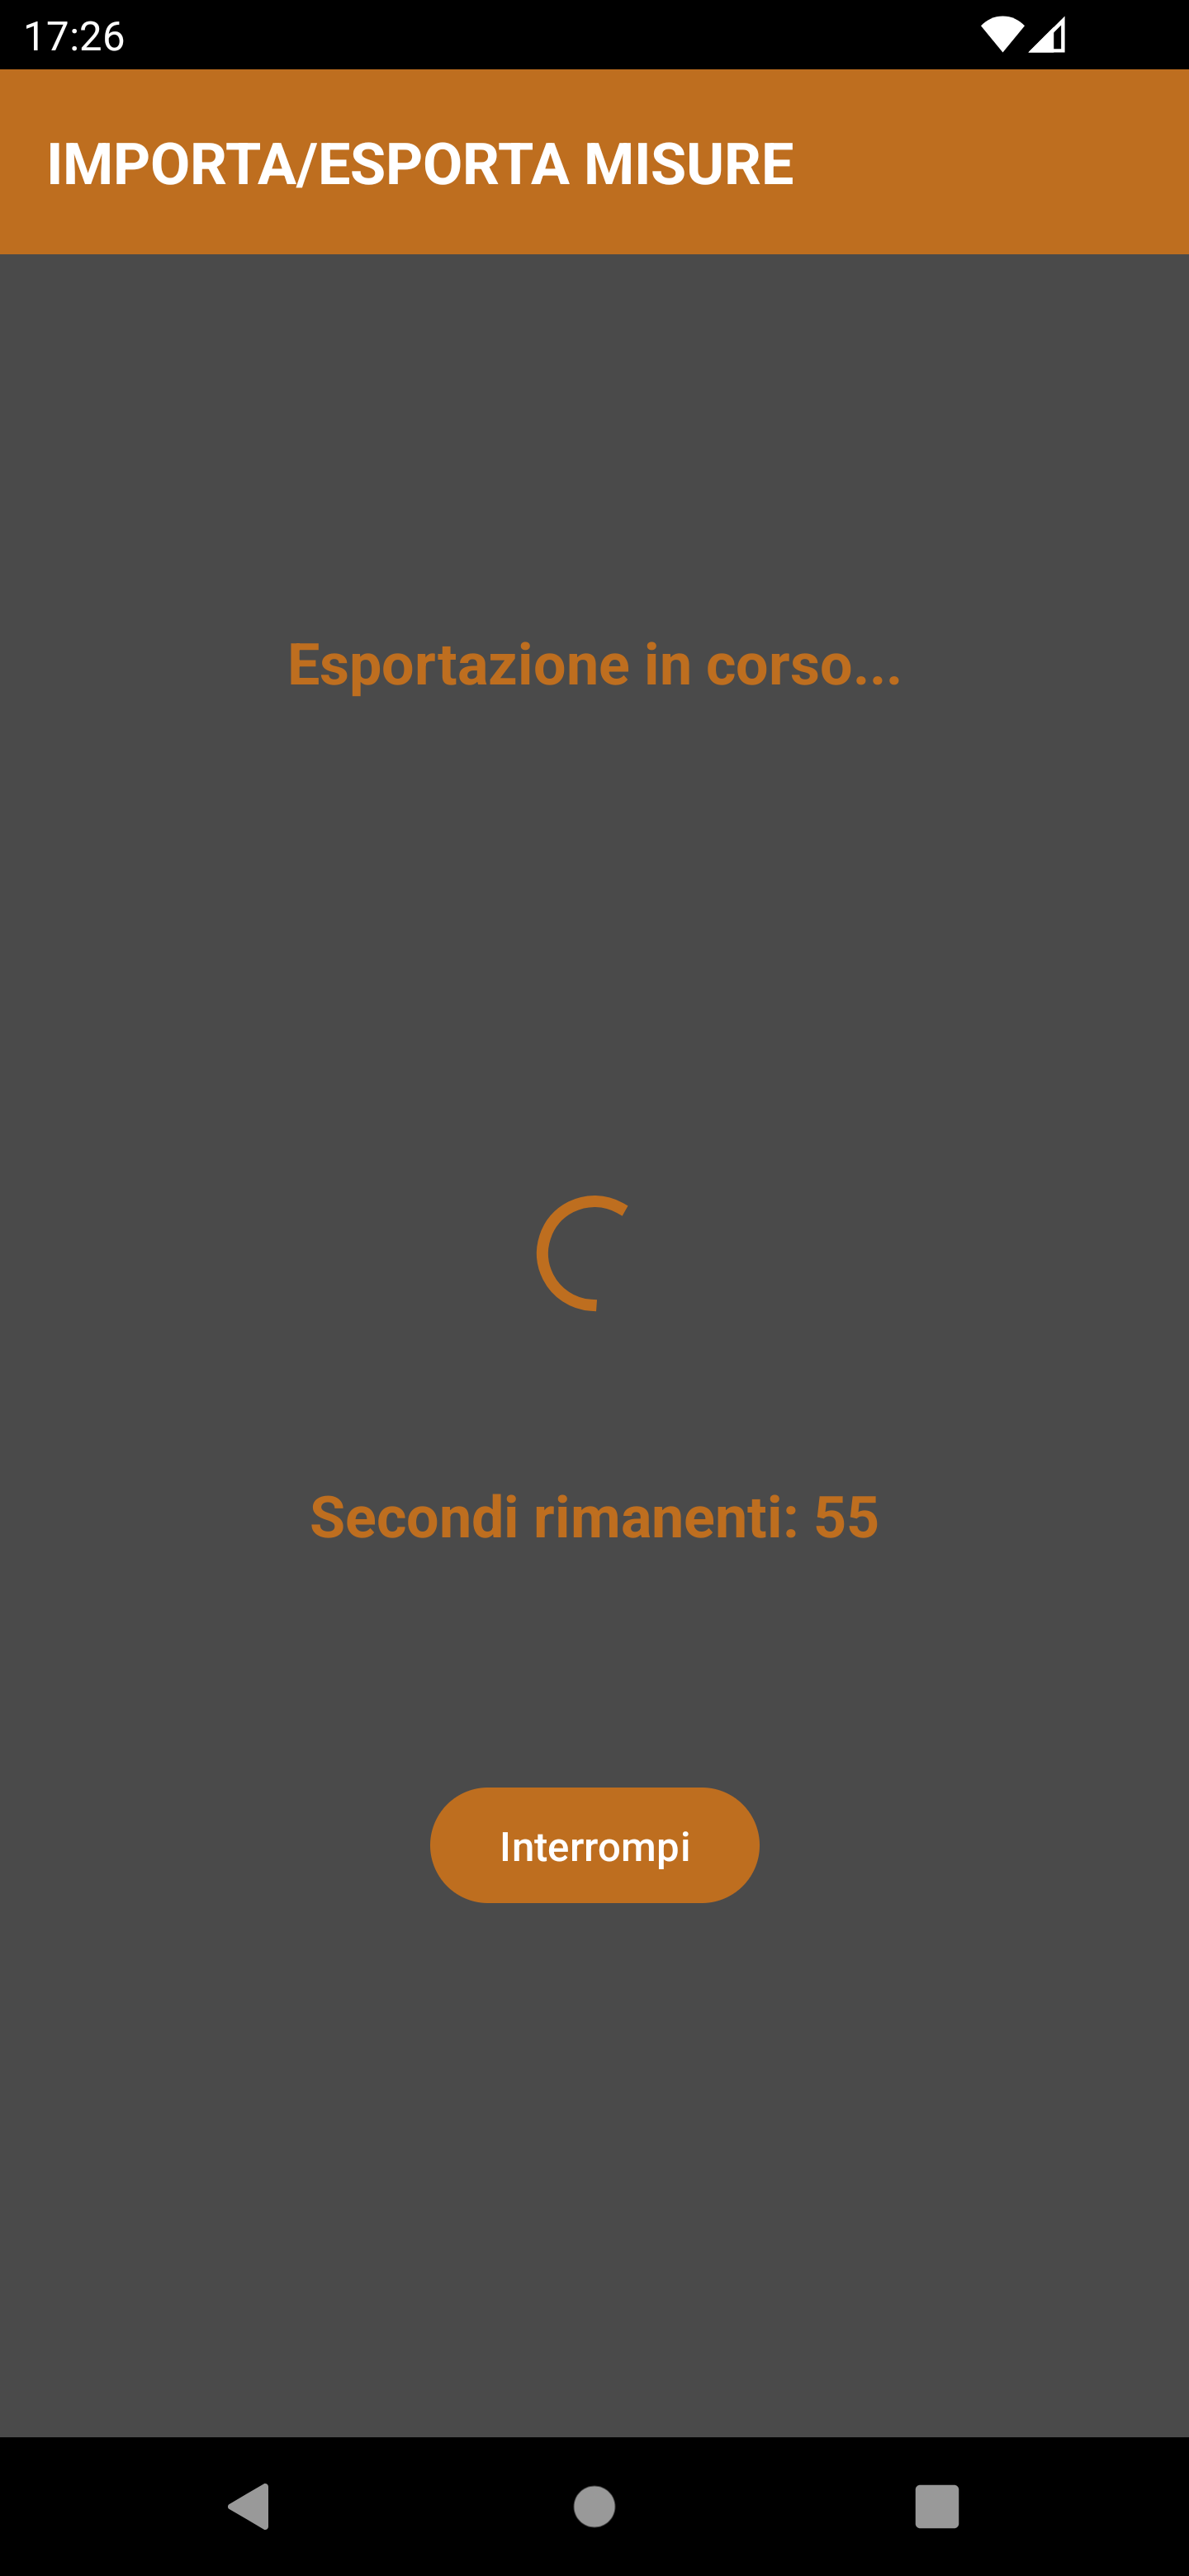
\includegraphics[width=0.3\textwidth]{img/exportBluetooth.png}%
        \label{fig:exportBluetooth}%
        }%

    \caption{Schermata di scambio dati}
\end{figure}
\section{Dettagli implementativi}
\subsection{Permessi}
\label{sec:permessi}
Da Android 11 le richieste dei permessi sono cambiate\footnote{\href{https://developer.android.com/about/versions/11/privacy/permissions?hl=en\#dialog-visibility}{Permissions updates in Android 11 - Android Developers}}. Per aggirare questo problema si è deciso di mostrare un dialog che, in caso l'utente vieti i permessi oltre il nuovo limite imposto, gli notifica l'assenza dei permessi e lo indirizza alle impostazioni dell'applicazione per autorizzarli manualmente. \\
Tale procedura è stata applicata per le richieste dei permessi di posizione, notifica, bluetooth e microfono. Per i permessi iniziali di posizione, dato che sono fondamentali per il funzionamento minimale dell'applicazione, l'utente è forzato a fornire i permessi nelle impostazioni per proseguire con l'utilizzo dell'applicazione.
\subsection{Mappa}
Per la visualizzazione della mappa, sono utilizzate le \texttt{API} di \texttt{Google Maps} ed è implementata nella Main Activity tramite un fragment di classe \texttt{SupportMapFragment}. Viene inizializzata, tramite la funzione \texttt{loadMap}, dopo che l'utente ha fornito i permessi di posizione. \\
Per localizzare l'utente sulla mappa viene utilizzato un \texttt{LocationListener} che viene aggiornato ogni due secondi e il cui ciclo di vita è legato a quello di \texttt{resume} e \texttt{stop} della Main Activity
\subsubsection{Griglia}
La griglia è implementata tramite oggetti della classe \texttt{Polygon} di Google Maps che vanno a formare i singoli riquadri. È generata dalla funzione \texttt{drawGridOnMap} della classe \texttt{Map}.\\
Per avere una griglia fissata alla mappa e non allo schermo in modo da avere la griglia indipendente dal movimento della mappa, si è considerata una coordinata canonica di partenza dalla quale si calcolano le posizioni di tutti i riquadri della griglia. \\
Quindi per calcolare la posizione di un riquadro in cui è compresa una determinata coordinata (\texttt{lat}, \texttt{lon}), viene calcolata la coordinata del vertice in alto a sinistra tramite la funzione \texttt{generateTopLeftPoint}, e da lì viene disegnato il resto del riquadro. Tale funzione genera il punto tramite le seguenti formule:
\begin{equation*}
    \texttt{lat}_{\texttt{tlPoint}} = \left \lceil \dfrac{\texttt{lat} - \texttt{lat}_{\texttt{start}}}{\texttt{offset}} \right \rceil \cdot \texttt{offset}
\end{equation*}
\begin{equation*}
    \texttt{lon}_{\texttt{tlPoint}} = \left \lfloor \dfrac{\texttt{lon} - \texttt{lon}_{\texttt{start}}}{\texttt{offset}} \right \rfloor \cdot \texttt{offset}
\end{equation*}
Dove $\texttt{lat}_{\texttt{tlPoint}}$ e $\texttt{lon}_{\texttt{tlPoint}}$ sono le coordinate del punto in alto a sinistra del riquadro che si sta calcolando. \texttt{Offset} è la lunghezza di un lato di un riquadro ed è calcolato dal metodo \texttt{metersToOffset} che prende in input la grandezza di un riquadro in base allo zoom (\texttt{meters}) e la converte in gradi usando la proporzione $1^{\circ} \texttt{ lat}/\texttt{lon} = 111km$ circa. $\texttt{Lat}_{\texttt{start}}$ e $\texttt{lon}_{\texttt{start}}$ sono le coordinate della posizione canonica presa come punto di riferimento, ovvero il punto $(0,0)$. \\
Una volta definite le funzioni ausiliarie, per rappresentare la griglia viene preso in considerazione il punto in alto a sinistra dello schermo del dispositivo e viene generato il riquadro in cui è compreso. Successivamente viene calcolata l'area dello schermo del dispositivo e si generano riquadri adiacenti finché lo schermo riesce a visualizzarli, prima orizzontalmente poi verticalmente. Ogni riquadro viene aggiunto ad una lista dei poligoni in modo da poter essere richiamato successivamente.\\
Per gestire la colorazione di un riquadro, viene utilizzata la funzione \texttt{getQuality}, che prendendo in input le medie dei tre tipi di misurazione in quel riquadro (limitando eventualmente il numero di misure da prendere in considerazione per la media in base al limite specificato dall'utente), li confronta con le soglie pessime e ottimali (di default o impostate dall'utente) e associa ad ogni tipo di misurazione il colore rosso se la media si trova sotto la soglia pessima, verde se si trova sopra la soglia ottimale e giallo se si trova in mezzo. \\ \\
L'interazione con i riquadri è implementata tramite un listener della mappa, che ad ogni tocco restituisce la posizione in cui si è premuto e questa viene usata per ottenere il poligono relativo. Successivamente prende le misure in quel riquadro e fornisce le informazioni all'utente tramite dei dialog. \\
Inizialmente viene mostrato un dialog con informazioni generali sulle misure presenti nel riquadro. Premendo su "\texttt{Mostra di più}" viene creato un ulteriore dialog che mostra la lista di misure. Selezionando una misura si viene portati in un ultimo dialog che mostra nello specifico tutte le informazioni della misura selezionata con la possibilità di cancellarla. La cancellazione avviene invocando il \texttt{DAO} del database e fornendo l'id della misura alla query di cancellazione.
\subsection{Notifica}
\label{sec:notifica}
La funzionalità di inviare una notifica se si entra in un riquadro senza misure recenti viene gestita nel metodo \texttt{listenerHandler} con parametro \texttt{isInFetchingMode} a \texttt{false}. \\
Per rilevare quando l'utente entra in un nuovo riquadro, viene confrontata la sua posizione presa dal \texttt{LocationListener} con l'ultima registrata controllando se le due posizioni si trovano in riquadri diversi. In caso affermativo viene chiamato il database per controllare se l'ultima misura in quel riquadro risale al giorno odierno e in caso negativo viene inviata una notifica per segnalare la mancanza.
\subsection{Sensori}
La gestione dei sensori avviene nella classe \texttt{Sensor} che implementa i metodi di misurazione per ciascuno dei tre componenti. \\
Le misurazioni LTE e Wi-Fi vengono effettuate instantaneamente, mentre per il calcolo del dB si campionano due misure del microfono nell'arco di tre secondi ignorando il primo perché non viene captato nulla. I valori registrati, essendo calcolati in ampiezza, vengono convertiti in dB con la funzione \texttt{fetchAmplitude}.
\pagebreak
\subsection{Metodi di misurazione} % Come effettua una misura, db ecc...
All'interno dell'applicazione è implementato un database locale con \texttt{Room} che immagazzina le misure registrate. Nel database una misura è memorizzata come oggetto della classe \texttt{Measure}, formata dai seguenti campi:
\begin{table}[H]
    \begin{tabular}{l|l}
        \textbf{Campo} & \textbf{Descrizione} \\
        \texttt{id} & ID della misura, autogenerato e univoco \\
        \texttt{timestamp} & Data e ora della misura \\
        \texttt{lat} & Latitudine della posizione \\
        \texttt{lon} & Longitudine della posizione \\
        \texttt{lte} & Valore LTE calcolato \\
        \texttt{wifi} & Valore Wi-Fi calcolato \\
        \texttt{db} & Valore dB calcolato \\
        \texttt{user\_id} & UUID univoco per ogni utente \\
        \texttt{imported} & True se la misura è importata, false se è stata effettuata dall'utente
    \end{tabular}
\end{table}
\noindent La creazione di una misura avviene nella funzione \texttt{addMeasurement} che crea un oggetto \texttt{Measure} e lo popola con l'orario e la posizione attuale, le misure registrate tramite la classe \texttt{Sensor}, l'UUID univoco dell'utente e impostando il flag \texttt{imported} a \texttt{false}. Successivamente lo importa nel database. Infine, in base al flag \texttt{isOutside} passato come parametro, che indica se la misura è stata effettuata al di fuori dell'area dello schermo, aggiorna o no la griglia.
\subsubsection{Periodic}
La funzionalità di scansione periodica è gestita nel metodo \texttt{periodicFetch} che, finché è attivo lo switch \texttt{periodic\_fetch} nelle impostazioni, effettua misure con un intervallo scelto dall'utente.
\subsubsection{Periodic in background}
La funzionalità viene gestita tramite il servizio \texttt{PeriodicFetchService}, la cui attivazione e disattivazione sono gestite dentro alla Main Activity in base allo switch \texttt{background\_periodic\_fetch} nelle impostazioni. \\
Il servizio, che permette all'applicazione di agire in background, invia una notifica fissa nella Status Bar che segnala che il servizio è in esecuzione e quante misure ha effettuato dall'avvio, successivamente effettua misure con un intervallo scelto dall'utente. \\
Durante il ciclo di vita del servizio, la mappa nel Main Activity viene oscurata.
\subsubsection{Automatic}
La funzionalità viene gestita nel metodo \texttt{listenerHandler} con parametro \texttt{isInFetchingMode} a \texttt{true}. Per rilevare quando l'utente entra in un nuovo riquadro, viene utilizzato lo stesso metodo utilizzato per la notifica (Capitolo \ref{sec:notifica}).
\subsection{Scambio di dati}
Lo scambio delle misure viene gestito nell'activity \texttt{SwapActivity}. \\
Il compito principale dell'activity è manipolare oggetti JSON per importare ed esportare misure nel database locale.
\subsubsection{Da file}
L'importazione è gestita lanciando un intent \texttt{ACTION\_OPEN\_DOCUMENT} per permettere all'utente di selezionare il file. Dopo la selezione, vengono ricavate le misure dal file JSON e importate nel database tramite la funzione \texttt{importData}. Per evitare di importare più volte la stessa misura, viene prima controllato che non siano già presenti nel database misure con lo stesso ID utente, orario e posizione. \\
L'esportazione è gestita dalla funzione \texttt{exportData} che prende tutte le misure, escludendo quelle importate, dal database e le inserisce in un file JSON con estensione \texttt{.mapc}. Successivamente lancia un intent \texttt{ACTION\_SEND} per permettere all'utente di condividere il file.
\subsubsection{Bluetooth}
Lo scambio dati con Bluetooth è implementato tramite un'architettura Client/Server dove chi esporta funge da Server e chi importa funge da Client. \\
Prima di tutto vengono controllati i permessi relativi al Bluetooth e, in caso non sia attivo, viene chiesto di attivarlo. \\
L'importazione è gestita a partire dalla funzione \texttt{btReceiveHandler} che inizia la scansione dei dispositivi nelle vicinanze che hanno l'esportazione attiva e, grazie ad un oggetto \texttt{BroadcastReceiver} che quando riceve l'intent \texttt{ACTION\_FOUND} relativo a un dispositivo rilevato, lo mostra all'utente aggiungendolo ad una lista di dispositivi rilevati, che viene aggiornata ad ogni ciclo di scansione rimuovendo i dispositivi non più rilevabili. Quando l'utente preme su un dispositivo, viene inizializzata la connessione istanziando un oggetto di classe \texttt{ConnectThread} che ferma la scansione dei dispositivi e crea un socket per la connessione utilizzando un UUID per identificare l'app. \\
Una volta ricevute le misure, in una stringa formato JSON, vengono importate tramite la funzione \texttt{importData}. \\
L'esportazione è gestita a partire dalla funzione \texttt{btDiscoverHandler} che, tramite un intent \texttt{ACTION\_REQUEST\_DISCOVERABLE}, richiede all'utente di attivare la discoverabilità per una durata impostata. Se l'utente accetta viene inizializzato il server istanziando un oggetto della classe \texttt{AcceptThread}, che crea un server socket con lo stesso UUID del lato client per ricevere connessioni e rimane in ascolto finché un dispositivo si connette o scade il tempo. Una volta accettata la connessione con un client, si connette al suo socket e chiude il server socket creato precedentemente. Successivamente viene creata e trasmessa al client una stringa formato JSON che contiene tutte le misure, eccetto quelle importate, aggiungendo in coda una stringa \texttt{-- END --} per segnalare al client quando la trasmissione della stringa è terminata. \\
Mentre l'esportazione è in corso, viene mostrato un fragment che implementa un countdown sincronizzato con la durata della discoverabilità decisa nelle impostazioni e un bottone per terminare l'esportazione instantaneamente. Al termine del countdown o alla chiusura manuale dell'esportazione la discoverabilità viene disattivata e il fragment viene nascosto.
\pagebreak
\section{Bug noti}
Di seguito vengono elencati, in ordine di gravità, i maggiori bug riscontrati durante lo sviluppo dell'applicazione, non risolti o aggirati.
\begin{enumerate}
    \item In base al dispositivo usato, si sono notati comportamenti diversi dati dalla diversa gestione di Android e dell'ottimizzazione dei processi.
    \begin{enumerate}
        \item Su dispositivo fisico OnePlus, il programma va in crash all'avvio perché l'applicazione va direttamente alla callback \texttt{onRequestPermissionResult} prima che l'utente possa fornire o rifiutare i permessi. Per ovviare a questo problema bisogna concederli manualmente dalle impostazioni.
    \end{enumerate}
    \item Su emulatore, durante la background periodic fetch, l'applicazione va in crash per timeout solo quando si rimane in MainActivity.
    \item A volte è possibile che non venga visualizzata la richiesta di permessi per il motivo citato nel Capitolo \ref{sec:permessi}. In tal caso è sufficiente riavviare l'applicazione per mostrare il dialog che rimanda alle impostazioni.
    \item Le misure vengono effettuate con un fuso orario fisso (UTC) e non viene modificato se il dispositivo cambia manualmente il fuso orario.
    \item Quando la mappa viene visualizzata con lo zoom minimo, la griglia non viene mostrata correttamente.
\end{enumerate}

\end{document}